\section{Álgebra de conjuntos}

%Dos conjuntos $A$ y $B$ se dicen \emph{disjuntos} si no tienen elementos en común, es decir $A\cap B=\emptyset$.
%
%
%Supongamos que 
%$$
%S=A\cup B, \; A\cap B=\emptyset.
%$$  Diremos que $S$ es la unión disjunta de $A$ y $B$ y se denota por $$S=A \sqcup B.$$ 



\subsection{Complementos, Diferencias y Diferencias Sim\'etricas}


En esta sección, consideraremos conjuntos que sean subconjuntos de un conjunto universo fijo $\uset.$



El \emph{complemento} $A^{C}$ de un conjunto $A$ es el conjunto de elementos que no pertenecen a $A$, es decir 
$$A^{C}=\set{x\in \uset \mid x \notin A}.$$



Algunos textos denotan $A^{C}$ tambi\'en como $A'$ o $\bar{A}.$ 



El \emph{complemento relativo} de un conjunto $B$ con respecto a un conjunto $A$ se define como 
$$
A\minus B = \set{x \mid x \in A, x \notin B}.
$$
De manera equivalente,	$A \minus B = A \cap B^{C}.$

El conjunto $A\minus B$ se lee \texttt{$A$ menos $B$.} Algunos textos lo denotan tambi\'en como $A-B.$  

La \emph{diferencia sim\'etrica} de los conjuntos $A$ y $B$ se define como $$A\symdif B=\left( A\cup B \right)\minus \left( A \cap B \right).$$



\begin{figure}
	\centering
	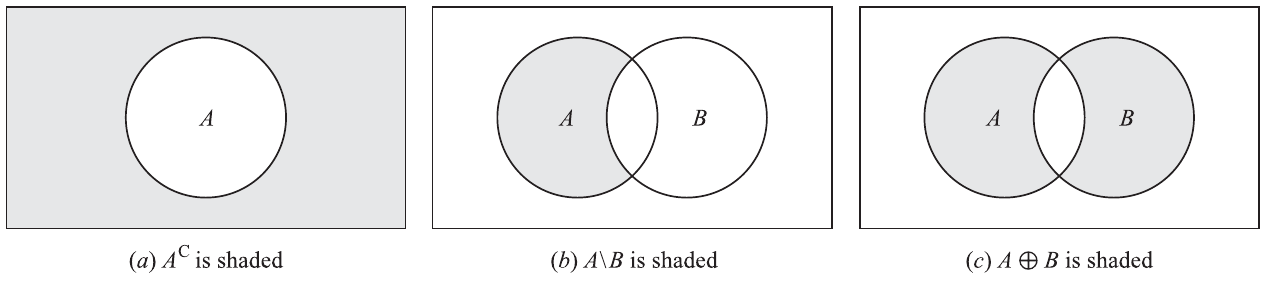
\includegraphics[width=10cm,keepaspectratio=true]{./md/venn_complemento.png}
	% venn_complemento.png: 0x0 pixel, 300dpi, 0.00x0.00 cm, bb=
	\caption{Complementos, diferencia y diferencia simétrica.}
	\label{fig:0104}
\end{figure}






\subsection{Conjuntos fundamentales}


Dos conjuntos $A$ y $B$ se dicen \emph{disjuntos} si no tienen elementos en común, es decir $A\cap B=\emptyset$.


Supongamos que 
$$
S=A\cup B, \; A\cap B=\emptyset.
$$  Diremos que $S$ es la unión disjunta de $A$ y $B$ y se denota por $$S=A \sqcup B.$$ 




En general $S$ es una unión disjunta de $P_{1}, P_{2},...,P_{n}$ si 
\begin{itemize}
	\item $\displaystyle S=P_{1}\cup P_{2}\cup...\cup P_{n}$ y
	\item $P_{i}\cap P_{j}=\emptyset$ siempre y cuando $i\neq j.$
\end{itemize}


En este caso, escribimos
$$
S=P_{1}\sqcup P_{2}\sqcup...\sqcup P_{n}.
$$



Diremos que $P_{1}, P_{2},...,P_{n}$ es sistema de conjuntos fundamentales para $\uset$ si
$$
\uset = P_{1}\sqcup P_{2}\sqcup...\sqcup P_{n}.
$$






\begin{figure}
	\centering
	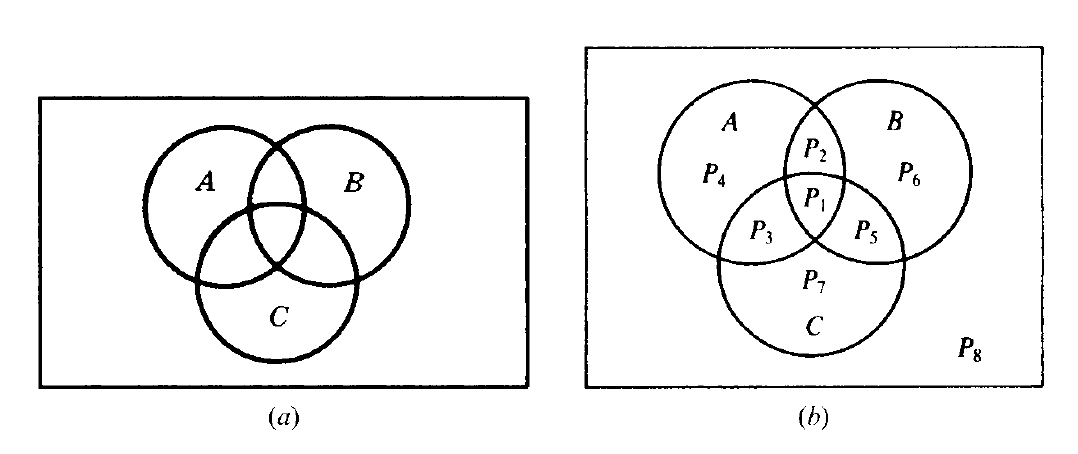
\includegraphics[width=10cm,keepaspectratio=true]{./md/sistema_fundamental.png}
	% sistema_fundamental.png: 0x0 pixel, 300dpi, 0.00x0.00 cm, bb=
	\label{fig:0105}
\end{figure}




\subsection{Álgebra de conjuntos, dualidad}


Los conjuntos bajo las operaciones de unión, intersección y complemento satisface varias leyes o identidad, que se enuncian en la siguiente tabla, y son similares a las leyes de lógica.



\begin{figure}
	\centering
	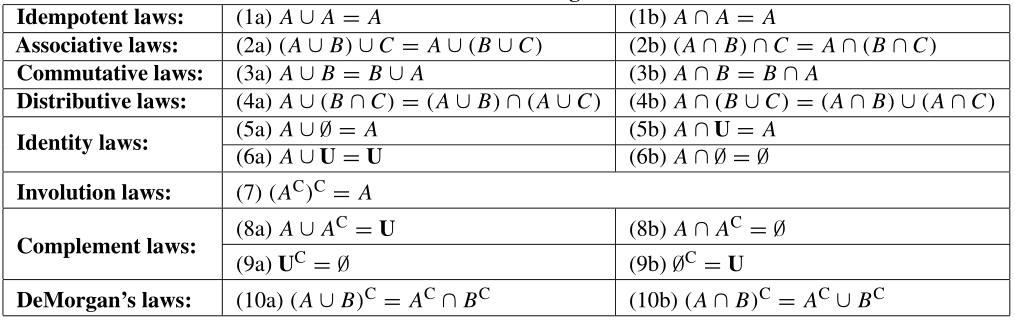
\includegraphics[width=11cm,keepaspectratio=true]{./md/leyes_conjuntos.png}
	\caption{Leyes de Conjuntos}
	\label{fig:leyesconjuntos}
\end{figure}




Cada ley de conjuntos se corresponde con una ley de lógica. Por ejemplo, la ley de DeMorgan:
\begin{align*}
	\left(A \cup B\right)^{C} &= \set{x \mid x\notin(A \cup B)}\\
	&= \set{x \mid x\notin A \wed x\notin B}\\
	&=A^{C}\cap B^{C}
\end{align*}



{Dualidad}
El \emph{principio de dualidad} establece que la equivalencia $E^{*}$ obtenida a partir de una ley de lógica $E$ reemplazando
\[ \cup, \cap, \uset, \emptyset\] por
\[ \cap, \cup, \emptyset, \uset\]
sigue siendo una ley de lógica.


A la proposición $E^{*}$ se le conoce como dual $E.$

